% fig_pipeline.tex - the pipelined datapath (pipelined/rtl/riscv_core.sv): the five stage
% modules, the four pipeline registers, forwarding, the hazard unit and the write-back bypass.
\documentclass[tikz,border=8pt]{standalone}
\usepackage[T1]{fontenc}
\usepackage{lmodern}
\usepackage[scaled=0.92]{helvet}
\renewcommand{\familydefault}{\sfdefault}
% rv32i_style.tex - shared TikZ styles for the single-cycle RV32I diagrams.
% Visual language:
%   thick border, blue fill  = holds state (clocked)
%   thin border, white fill  = combinational logic
%   green trapezium          = multiplexer (0/1 marks the input chosen by select)
%   dashed orange            = control signal;  solid navy = data
%   /32 on a wire            = bus width;       dot = wires joined
% Port names are the exact SystemVerilog port names of the module drawn.
\usetikzlibrary{arrows.meta, positioning, calc, fit, backgrounds, shapes.geometric, shapes.misc}

\definecolor{ink}{RGB}{31,56,100}
\definecolor{statefill}{RGB}{220,230,242}
\definecolor{muxdraw}{RGB}{56,118,59}
\definecolor{muxfill}{RGB}{226,239,218}
\definecolor{ctrl}{RGB}{197,90,17}
\definecolor{ctrlfill}{RGB}{252,232,216}
\definecolor{note}{RGB}{110,110,110}
\definecolor{tintIF}{RGB}{236,243,251}
\definecolor{tintID}{RGB}{240,247,235}
\definecolor{tintEX}{RGB}{255,246,229}
\definecolor{tintMEM}{RGB}{244,237,249}
\definecolor{tintWB}{RGB}{233,246,245}

\tikzset{
  >={Stealth[length=2.2mm,width=1.6mm]},
  wire/.style      = {draw=ink, line width=0.75pt},
  data/.style      = {wire, ->},
  ctl/.style       = {draw=ctrl, line width=0.75pt, dashed, dash pattern=on 3pt off 1.6pt, ->},
  ctlnoarrow/.style= {draw=ctrl, line width=0.75pt, dashed, dash pattern=on 3pt off 1.6pt},
  block/.style     = {draw=ink, line width=0.75pt, fill=white, rectangle, align=center,
                      inner sep=3pt, font=\small},
  state/.style     = {block, line width=1.8pt, fill=statefill},
  ctrlblock/.style = {block, draw=ctrl, fill=ctrlfill},
  muxst/.style     = {draw=muxdraw, fill=muxfill, line width=0.9pt},
  aluSt/.style     = {draw=ink, fill=white, line width=0.9pt},
  addr/.style      = {circle, draw=ink, fill=white, line width=0.75pt, inner sep=0.5pt,
                      minimum size=6.5mm, font=\large},
  stage/.style     = {draw=ink!70, rounded corners=6pt, line width=0.9pt},
  sig/.style       = {font=\scriptsize\ttfamily, text=ink, inner sep=1.2pt},
  csig/.style      = {font=\scriptsize\ttfamily, text=ctrl, inner sep=1.2pt},
  wlbl/.style      = {font=\tiny, text=ink, inner sep=0.8pt},
  notetxt/.style   = {font=\scriptsize\itshape, text=note, align=left},
  mlbl/.style      = {font=\tiny\bfseries, text=muxdraw, inner sep=0pt},
  title/.style     = {font=\large\bfseries, text=ink},
  dot/.style       = {circle, fill=ink, inner sep=0pt, minimum size=4pt},
  cdot/.style      = {circle, fill=ctrl, inner sep=0pt, minimum size=4pt},
  portbox/.style   = {rectangle, fill=ink, inner sep=0pt, minimum size=4pt},
  cportbox/.style  = {rectangle, fill=ctrl, inner sep=0pt, minimum size=4pt},
  flag/.style      = {sig, draw=ink, fill=white, rounded corners=1.5pt, inner sep=1.5pt},  % net label
  stub/.style      = {ctl},                                                                 % named select input
}

% Two-line block label: module name, then "instance : module".
\newcommand{\blk}[2]{\textbf{#1}\\[-1pt]{\scriptsize\ttfamily #2}}
% Same with a two-line name.
\newcommand{\blkII}[3]{\textbf{#1}\\[-2pt]\textbf{#2}\\[-1pt]{\scriptsize\ttfamily #3}}

% Bus-width mark on a horizontal wire: \wmark{(x,y)}{32}
\newcommand{\wmark}[2]{%
  \draw[draw=ink, line width=0.6pt] ($#1+(-0.07,-0.13)$) -- ($#1+(0.07,0.13)$);
  \node[wlbl, above] at ($#1+(0,0.1)$) {#2};}
% Bus-width mark on a vertical wire: \wmarkv{(x,y)}{32}
\newcommand{\wmarkv}[2]{%
  \draw[draw=ink, line width=0.6pt] ($#1+(-0.13,-0.07)$) -- ($#1+(0.13,0.07)$);
  \node[wlbl, right] at ($#1+(0.1,0)$) {#2};}

% Multiplexer, inputs on the left, output on the right.
% \muxR{name}{x}{y}{height}: defines (name-out), (name-top), (name-bot), (name-l) (left x).
\newcommand{\muxR}[4]{%
  \draw[muxst] ($(#2,#3)+(-0.28,-#4/2)$) -- ($(#2,#3)+(-0.28,#4/2)$)
               -- ($(#2,#3)+(0.28,#4/2-0.28)$) -- ($(#2,#3)+(0.28,-#4/2+0.28)$) -- cycle;
  \coordinate (#1-out) at ($(#2,#3)+(0.28,0)$);
  \coordinate (#1-top) at ($(#2,#3)+(0,#4/2-0.14)$);
  \coordinate (#1-bot) at ($(#2,#3)+(0,-#4/2+0.14)$);
  \coordinate (#1-l)   at ($(#2,#3)+(-0.28,0)$);}

% ALU shape (notched trapezium), inputs a (upper) and b (lower) on the left.
% \aluR{name}{x}{y}{height}: defines (name-a), (name-b), (name-out), (name-op) (top edge).
\newcommand{\aluR}[4]{%
  \draw[aluSt] ($(#2,#3)+(-0.65,#4/2)$) -- ($(#2,#3)+(0.65,#4/4)$) -- ($(#2,#3)+(0.65,-#4/4)$)
               -- ($(#2,#3)+(-0.65,-#4/2)$) -- ($(#2,#3)+(-0.65,-0.28)$) -- ($(#2,#3)+(-0.35,0)$)
               -- ($(#2,#3)+(-0.65,0.28)$) -- cycle;
  \coordinate (#1-a)   at ($(#2,#3)+(-0.65,#4*0.3)$);
  \coordinate (#1-b)   at ($(#2,#3)+(-0.65,-#4*0.3)$);
  \coordinate (#1-out) at ($(#2,#3)+(0.65,0)$);
  \coordinate (#1-op)  at ($(#2,#3)+(0,#4*0.375)$);
  \coordinate (#1-c)   at ($(#2,#3)+(0.12,0)$);}

% Ports on a stage boundary. \inport{x}{y}{name}{width}  (label to the left)
% The width may be empty (1-bit port); it is expanded first so \foreach variables work.
\newcommand{\portw}[1]{\edef\pwtmp{#1}\ifx\pwtmp\empty\else\,[\pwtmp]\fi}
\newcommand{\inport}[4]{%
  \node[portbox] at (#1,#2) {};
  \node[sig, anchor=east] at ($(#1,#2)+(-0.12,0)$) {#3\portw{#4}};}
\newcommand{\cinport}[4]{%
  \node[cportbox] at (#1,#2) {};
  \node[csig, anchor=east] at ($(#1,#2)+(-0.12,0)$) {#3\portw{#4}};}
\newcommand{\outport}[4]{%
  \node[portbox] at (#1,#2) {};
  \node[sig, anchor=west] at ($(#1,#2)+(0.12,0)$) {#3\portw{#4}};}
\newcommand{\coutport}[4]{%
  \node[cportbox] at (#1,#2) {};
  \node[csig, anchor=west] at ($(#1,#2)+(0.12,0)$) {#3\portw{#4}};}
% Control input port on the top edge (label above).
\newcommand{\ctopport}[4]{%
  \node[cportbox] at (#1,#2) {};
  \node[csig, anchor=south] at ($(#1,#2)+(0,0.1)$) {#3\portw{#4}};}
% Data input port on the top edge (label above).
\newcommand{\topport}[4]{%
  \node[portbox] at (#1,#2) {};
  \node[sig, anchor=south] at ($(#1,#2)+(0,0.1)$) {#3\portw{#4}};}

% Legend strip. \legend{x}{y}
\newcommand{\legend}[2]{%
  \begin{scope}[shift={(#1,#2)}, font=\scriptsize]
    \node[state, minimum width=6mm, minimum height=3.5mm, inner sep=0pt] at (0,0) {};
    \node[anchor=west] at (0.45,0) {holds state};
    \node[block, minimum width=6mm, minimum height=3.5mm, inner sep=0pt] at (3.2,0) {};
    \node[anchor=west] at (3.65,0) {combinational};
    \draw[muxst] (6.2,-0.25) -- (6.2,0.25) -- (6.5,0.1) -- (6.5,-0.1) -- cycle;
    \node[anchor=west] at (6.6,0) {multiplexer};
    \draw[data] (8.7,0) -- (9.4,0); \node[anchor=west] at (9.45,0) {data};
    \draw[ctl] (10.4,0) -- (11.1,0); \node[anchor=west] at (11.15,0) {control};
    \node[portbox] at (12.6,0) {}; \node[anchor=west] at (12.7,0) {module port};
    \draw[wire] (14.6,0) -- (15.3,0); \draw[draw=ink, line width=0.6pt] (14.88,-0.13) -- (15.02,0.13);
    \node[wlbl] at (14.95,0.24) {32}; \node[anchor=west] at (15.35,0) {bus width};
  \end{scope}}

\begin{document}
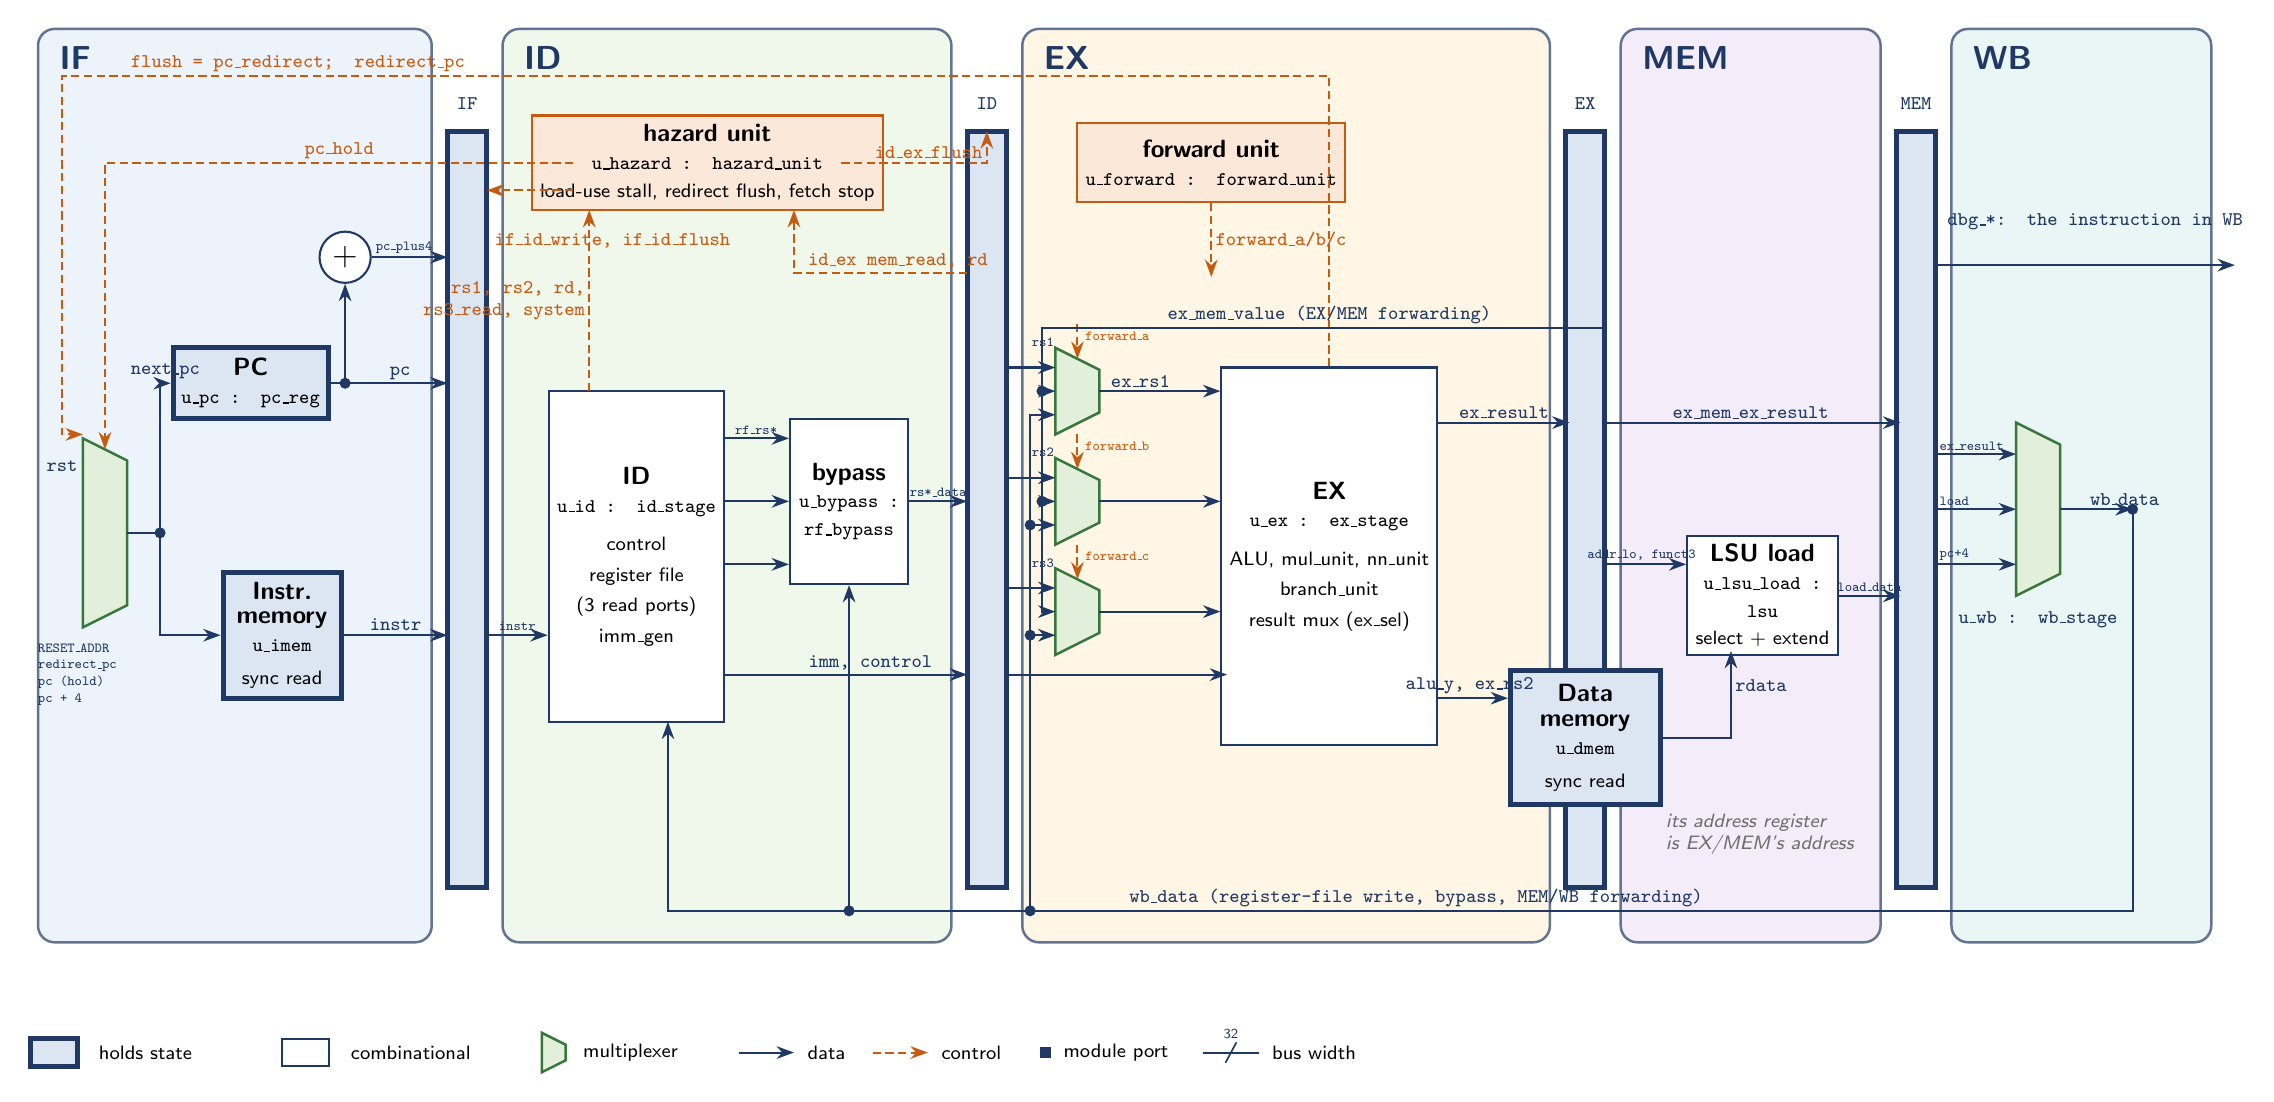
\begin{tikzpicture}
  % ---- stages (shaded) and pipeline registers (thick bars) ----
  \draw[stage, fill=tintIF]  (0,1)    rectangle (5.0,12.6);
  \draw[stage, fill=tintID]  (5.9,1)  rectangle (11.6,12.6);
  \draw[stage, fill=tintEX]  (12.5,1) rectangle (19.2,12.6);
  \draw[stage, fill=tintMEM] (20.1,1) rectangle (23.4,12.6);
  \draw[stage, fill=tintWB]  (24.3,1) rectangle (27.6,12.6);
  \foreach \x/\n in {0.15/IF, 6.05/ID, 12.65/EX, 20.25/MEM, 24.45/WB}
    \node[title, anchor=north west] at (\x,12.5) {\n};
  \foreach \x/\n in {5.45/IF/ID, 12.05/ID/EX, 19.65/EX/MEM, 23.85/MEM/WB} {
    \node[state, minimum width=5mm, minimum height=96mm, inner sep=0pt] at (\x,6.5) {};
    \node[sig, font=\scriptsize\bfseries\ttfamily] at (\x,11.65) {\n};
  }

  % ---- IF ----
  \muxR{npc}{0.85}{6.2}{2.4}
  \node[sig, anchor=east] at (0.55,7.05) {rst};
  \node[mlbl, anchor=west] at (0.6,7.1) {};
  \node[sig, font=\tiny\ttfamily, anchor=west, align=left] at (-0.05,4.4) {RESET\_ADDR\\redirect\_pc\\pc (hold)\\pc + 4};
  \node[state, minimum width=13mm, minimum height=9mm] (pc) at (2.7,8.1) {\blk{PC}{u\_pc : pc\_reg}};
  \node[state, minimum width=15mm, minimum height=16mm] (im) at (3.1,4.9)
       {\blkII{Instr.}{memory}{u\_imem}\\[1pt]{\scriptsize sync read}};
  \node[addr] (p4) at (3.9,9.7) {+};
  \draw[data] (npc-out) -- (1.55,6.2) |- node[sig, above, pos=0.75] {next\_pc} (pc.west);
  \draw[data] (1.55,6.2) |- (im.west);
  \node[dot] at (1.55,6.2) {};
  \draw[data] (pc.east) -- (5.2,8.1);
  \node[sig, above] at (4.6,8.1) {pc};
  \draw[data] (3.9,8.1) -- (p4.south);
  \node[dot] at (3.9,8.1) {};
  \draw[data] (p4.east) -- (5.2,9.7);
  \node[sig, font=\tiny\ttfamily, above] at (4.65,9.7) {pc\_plus4};
  \draw[data] (im.east) -- node[sig, above] {instr} (5.2,4.9);

  % ---- ID ----
  \node[block, minimum width=22mm, minimum height=42mm] (id) at (7.6,5.9)
       {\blk{ID}{u\_id : id\_stage}\\[3pt]{\scriptsize control}\\{\scriptsize register file}\\{\scriptsize (3 read ports)}\\{\scriptsize imm\_gen}};
  \node[block, minimum width=15mm, minimum height=21mm] (bp) at (10.3,6.6)
       {\blk{bypass}{u\_bypass :}\\[-1pt]{\scriptsize\ttfamily rf\_bypass}};
  \draw[data] (5.7,4.9) -- node[sig, font=\tiny\ttfamily, above] {instr} (id.west |- 0,4.9);
  \foreach \y/\s in {7.4/rs1, 6.6/rs2, 5.8/rs3}
    \draw[data] (id.east |- 0,\y) -- (bp.west |- 0,\y);
  \node[sig, font=\tiny\ttfamily, above] at (9.12,7.4) {rf\_rs*};
  \draw[data] (bp.east) -- node[sig, font=\tiny\ttfamily, above] {rs*\_data} (11.8,6.6);
  \draw[data] (id.east |- 0,4.4) -- node[sig, above, pos=0.6] {imm, control} (11.8,4.4);

  % ---- hazard unit ----
  \node[ctrlblock, minimum width=34mm, minimum height=12mm] (hz) at (8.5,10.9)
       {\blk{hazard unit}{u\_hazard : hazard\_unit}\\[-1pt]{\scriptsize load-use stall, redirect flush, fetch stop}};
  \draw[ctl] (7.0,8.0) -- node[csig, left, align=right] {rs1, rs2, rd,\\rs3\_read, system} (7.0,10.3);
  \draw[ctl] (11.8,9.5) -- node[csig, above, pos=0.4] {id\_ex mem\_read, rd} (9.6,9.5) -- (9.6,10.3);
  \draw[ctl] (6.8,10.9) -| node[csig, above, pos=0.25] {pc\_hold} (npc-top);
  \draw[ctl] (6.8,10.55) -- (5.7,10.55);
  \node[csig, anchor=north west] at (5.75,10.05) {if\_id\_write, if\_id\_flush};
  \draw[ctl] (10.2,10.9) -| node[csig, above, pos=0.3] {id\_ex\_flush} (12.05,11.3);

  % ---- EX: forwarding muxes, forward unit, ex_stage ----
  % each mux: top input from ID/EX, middle from EX/MEM, bottom from MEM/WB
  \foreach \n/\y/\s/\f in {fa/8.0/rs1/forward\_a, fb/6.6/rs2/forward\_b, fc/5.2/rs3/forward\_c} {
    \muxR{\n}{13.2}{\y}{1.1}
    \draw[data] (12.3,\y+0.3) -- (12.92,\y+0.3);
    \node[sig, anchor=east, font=\tiny\ttfamily] at (12.95,\y+0.62) {\s};
    \draw[ctl] (13.2,\y+0.85) -- (\n-top);
    \node[csig, anchor=south west, font=\tiny\ttfamily] at (13.25,\y+0.6) {\f};
  }
  \node[ctrlblock, minimum width=26mm, minimum height=10mm] (fw) at (14.9,10.9)
       {\blk{forward unit}{u\_forward : forward\_unit}};
  \draw[ctl] (fw.south) -- node[csig, right] {forward\_a/b/c} (14.9,9.45);
  \node[block, minimum width=26mm, minimum height=48mm] (ex) at (16.4,5.9)
       {\blk{EX}{u\_ex : ex\_stage}\\[3pt]{\scriptsize ALU, mul\_unit, nn\_unit}\\{\scriptsize branch\_unit}\\{\scriptsize result mux (ex\_sel)}};
  \foreach \n in {fa, fb, fc} \draw[data] (\n-out) -- (ex.west |- \n-out);
  \node[sig, above] at (14.0,8.0) {ex\_rs1};
  \draw[data] (12.3,4.4) -- (15.1,4.4);
  \draw[data] (ex.east |- 0,7.6) -- node[sig, above] {ex\_result} (19.45,7.6);
  % redirect back to IF
  \draw[ctl] (ex.north) -- (16.4,12.0) -| (0.3,7.45) -- (0.57,7.45);
  \node[csig, anchor=south] at (3.3,12.0) {flush = pc\_redirect;\ \ redirect\_pc};

  % ---- the data memory: the access is issued at the end of EX ----
  \node[state, minimum width=19mm, minimum height=17mm] (dm) at (19.65,3.6)
       {\blkII{Data}{memory}{u\_dmem}\\[1pt]{\scriptsize sync read}};
  \draw[data] (ex.east |- 0,4.1) -- node[sig, above, pos=0.45] {alu\_y, ex\_rs2} (dm.west |- 0,4.1);
  \node[notetxt, anchor=north west] at (20.55,2.75) {its address register\\is EX/MEM's address};

  % ---- MEM ----
  \node[block, minimum width=17mm, minimum height=14mm] (ll) at (21.9,5.4)
       {\blk{LSU load}{u\_lsu\_load :}\\[-1pt]{\scriptsize\ttfamily lsu}\\[-1pt]{\scriptsize select + extend}};
  \draw[data] (dm.east) -| node[sig, right, pos=0.8] {rdata} (21.5,4.7);
  \draw[data] (19.9,5.8) -- node[sig, font=\tiny\ttfamily, above, pos=0.45] {addr\_lo, funct3} (ll.west |- 0,5.8);
  \draw[data] (ll.east) -- node[sig, font=\tiny\ttfamily, above] {load\_data} (23.65,5.4);
  \draw[data] (19.9,7.6) -- (23.65,7.6);
  \node[sig, above] at (21.75,7.6) {ex\_mem\_ex\_result};

  % ---- WB ----
  \muxR{wb}{25.4}{6.5}{2.2}
  \node[sig, anchor=north] at (25.4,5.25) {u\_wb : wb\_stage};
  \foreach \y in {7.2, 6.5, 5.8} \draw[data] (24.1,\y) -- (wb-l |- 0,\y);
  \node[sig, font=\tiny\ttfamily, anchor=south west] at (24.1,7.2) {ex\_result};
  \node[sig, font=\tiny\ttfamily, anchor=south west] at (24.1,6.5) {load};
  \node[sig, font=\tiny\ttfamily, anchor=south west] at (24.1,5.8) {pc+4};
  \draw[data] (wb-out) -- (26.6,6.5);
  \node[sig, above] at (26.5,6.5) {wb\_data};
  \node[dot] at (26.6,6.5) {};
  % wb_data: register-file write port and bypass (ID), and forwarding (EX)
  \draw[data] (26.6,6.5) -- (26.6,1.4) -| (8.0,3.8);
  \draw[data] (10.3,1.4) -- (bp.south);
  \node[dot] at (10.3,1.4) {};
  \draw[data] (12.6,1.4) -- (12.6,7.7) -- (12.92,7.7);
  \draw[data] (12.6,6.3) -- (12.92,6.3);  \node[dot] at (12.6,6.3) {};
  \draw[data] (12.6,4.9) -- (12.92,4.9);  \node[dot] at (12.6,4.9) {};
  \node[dot] at (12.6,1.4) {};
  \node[sig, above] at (17.5,1.4) {wb\_data (register-file write, bypass, MEM/WB forwarding)};
  % EX/MEM forwarding
  \draw[data] (19.9,8.8) -- (12.75,8.8) -- (12.75,5.2) -- (12.92,5.2);
  \draw[data] (12.75,8.0) -- (12.92,8.0);  \node[dot] at (12.75,8.0) {};
  \draw[data] (12.75,6.6) -- (12.92,6.6);  \node[dot] at (12.75,6.6) {};
  \node[sig, above] at (16.4,8.8) {ex\_mem\_value (EX/MEM forwarding)};
  % debug
  \draw[data] (24.1,9.6) -- (27.9,9.6);
  \node[sig, anchor=west, align=left] at (24.2,10.15) {dbg\_*: the instruction in WB};

  \legend{0.2}{-0.4}
\end{tikzpicture}
\end{document}
